% Chapter 1

\chapter{Prediction} % Write in your own chapter title
\label{Chapter3}
\lhead{Chapter3. \emph{Prediction}} % Write in your own chapter title to set the page header

Prediction is defined as duplication of the information contained in a macro-block using previously coded data. This duplicated information is subtracted from the macro-block to form a residual. There are 2 types of prediction.

\begin{itemize}
	\item Intra-Prediction
	\item Inter-Prediction
\end{itemize}

% ref of intra+prediction paper
\subsection{Intra-Prediction}
Intra-prediction utilizes the space dependency to compress the video. The frames which are intra coded using intra-prediction are called I-frames. Following are the possible prediction modes:
\begin{itemize}
	\item \textbf{4x4 luma:} having 9 directional modes and is suitable for macro blocks that has lot of details
	\item \textbf{8x8 luma:} having 9 directional modes and is for high profiles only.
	\item \textbf{16x16 luma:} having 4 directional modes that is suitable for macro block with smoother area
	\item \textbf{8x8 chroma:} 4 possible prediction modes and used for chrominance components
\end{itemize}
In our model, 4x4 luma prediction and 8x8 chroma prediction is being implemented.

\subsubsection{4x4 Luma Prediction}
For this type of prediction, each macro block that is of \textbf{16x16} (256 pixels each of which is 8 bit wide) is divided into \textbf{4x4} block (16 pixels). Figure \ref{fig:4x4xluma} shows the reference samples for 4x4 luma prediction. 4 pixels \textbf{A,B,C,D} (adjacent to current block) of block \textbf{a}  on top of current block, pixels \textbf{E,F,G,H} of block \textbf{b} on top right corner, \textbf{I,J,K,L} of block \textbf{c} at adjacent left of current block and 1 pixel \textbf{M} of \textbf{d} block on top left corner are used for prediction of 16 pixels in the current block.

\begin{figure}[htbp]
	\centering
	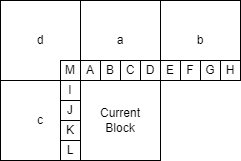
\includegraphics[width = 2.5in]{./Figures/4x4luma.png}
	\rule{35em}{0.5pt}
	\caption{Reference samples for 4x4 Luma}
	\label{fig:4x4xluma}
\end{figure}

There are total 9 prediction modes that are supported in this prediction. Major modes that are implemented in our model are as follows:

\begin{itemize}
	\item \textbf{Mode 0 (Vertical):} The predicted block is constructed by using upper samples A,B,C,D of block ‘a’ as shown in figure \ref{fig:3modes}. They are extrapolated vertically. It is suitable to predict vertical edges in the block.
	\item \textbf{Mode 1 (Horizontal):} In this mode, left samples I,J,K,L of block c are used. They are extrapolated horizontally and is suitable for horizontal edges. It can be seen in figure \ref{fig:3modes}.
	\item \textbf{Mode 2 (DC):} It utilizes average of all adjacent samples (A to D and I to L) to form the prediction of current block. It is suitable for smooth areas. Its process is shown in figure \ref{fig:3modes}.

\end{itemize}
	 
For the details of remaining modes refer to [give ref to richardson book here]. Figure \ref{fig:3modes} display the above 3 prediction modes. To create a predict sample, every color stands for a particular formula. The encoder determines each prediction direction's cost by finishing processing for all of the prediction directions, then outputs the one with the lowest cost.

\begin{figure}[htbp]
	\centering
	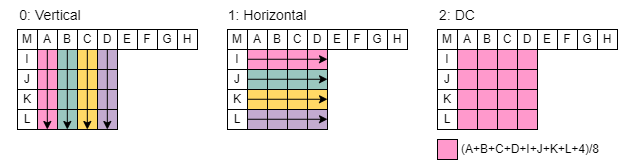
\includegraphics[width = 4in]{./Figures/3modes.png}
	\rule{35em}{0.5pt}
	\caption{Major Modes for 4x4 Luma Prediction}
	\label{fig:3modes}
\end{figure}

\subsubsection{8x8 Chroma Prediction}
This type of prediction applies on chrominance components. It is similar to 16x16 luma prediction which can be referred in [Richardson book] except the block size is 8x8 and there is different order of mode number which are:

\begin{itemize}
	\item Mode 0: DC
	\item Mode 1: Horizontal
	\item Mode 2: Vertical
	\item Mode 3: Plane
\end{itemize}

The working of first 3 modes in similar to mode 2,1,0 of 4x4 luma prediction respectively. For details of Plane mode refer to [Richardson book]. The Implemented mode in our model is DC. These modes are shown in the figure \ref{fig:8x8modes}.

\begin{figure}[htbp]
	\centering
	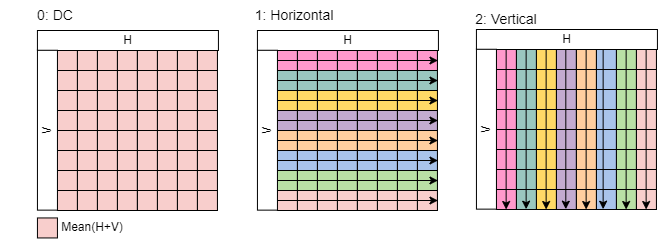
\includegraphics[width = 4in]{./Figures/8x8modes.png}
	\rule{35em}{0.5pt}
	\caption{Major Modes for 8x8 Chroma Prediction}
	\label{fig:8x8modes}
\end{figure}

[Explain the hardware architecture of Intra prediction if possible]

\subsection{Inter-Prediction}
The process of predicting a block of luma and chroma samples from a reference picture that has been previously been coded and transmitted i.e. exploits temporal redundancy between successive frames. For this a prediction region is selected, a prediction block is generated and then it is subtracted from original block of samples to form a residual. This is then coded and transmitted. Reference pictures are stored in Decoded Picture Buffer. The offset between position of current block and search region in the reference picture is called motion vector. This prediction is also known as \textbf{Motion Estimation} [ref of ppr Low power techniques]. It has the capability of extracting true motion information thus enhancing the quality of displayed images in video enhancement systems. The preferred technique for motion estimation is the \textbf{Block Matching (BM)} Technique. 

\subsubsection{Block Matching Technique}
This method divides the current frame into non-overlapping NxN macro-blocks and seeks out the block from the reference frame that most closely resembles the current block within a specified search range. The Sum of Absolute Difference (SAD), which is appropriate for hardware implementations, is the recommended block matching criterion.

In figure \ref{fig:mv}, \textbf{(x,y)} represents the location of the current frame. The search window in the reference frame is in \textbf{[-r,r]} region in both x and y directions. Both current and reference block lies within the range of search window. The SAD value is calculated by accumulating absolute differences of corresponding pixels in both current and reference blocks. A motion vector is the relative motion of current block in reference frame, they are specified in relative coordinates. Thus if \textbf{(x+a,y+b)} is the location of best matching block in reference frame, then \textbf{(a,b)} represents the motion vector. Motion Estimation is performed on luma component and resulting motion vectors are also used for chroma components.

\begin{figure}[htbp]
	\centering
	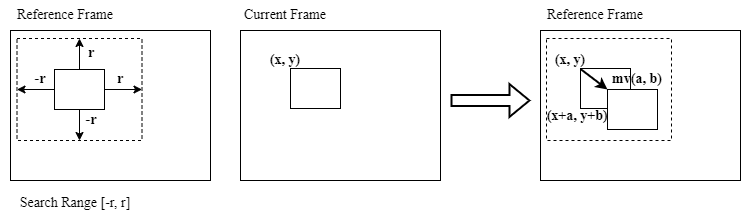
\includegraphics[width = 4in]{./Figures/mv.png}
	\rule{35em}{0.5pt}
	\caption{Motion Estimation using Block Matching}
	\label{fig:mv}
\end{figure}

There are several algorithms for Block Matching. Among them mostly used is \textbf{Full Search (FS)} algorithm. The SAD values for each search position within a specific search range are calculated by this approach to determine the reference block that most closely resembles the present block. It has the best performance related to other algorithms as it searches all the search locations in a given search range. But its computational complexity is high and its hardware consume a lot of power. For further improvement, instead of \textbf{fixed block size (FBS) FS ME} algorithm, \textbf{variable block size (VBS) FS ME} algorithm is incorporated. For details of FBS ME algorithm, refer to [that ppr]. VBS FS ME algorithm will be further explained in detail in next section.


\subsection{Hardware Architecture for Inter-Prediction}
